\section{Results}\label{sec:result}

Given a SPN primitive and $A$, the maximum S-boxes to be considered, we first generate graph $G$ according to Section \ref{algo:gen_G}. Applying our method in Section \ref{algo:find_ite_c_G}, we compute the weight growth of the best iterative characteristic. Applying our method in Section \ref{algo:find_ite_h_G}, we compute the weight growth of the best the best iterative hull. Comparing the two results, we show the strength of the clustering effect through a bar chart. 

\subsection{Results on Iterative Characteristics and Hulls}

We apply our algorithms in Section \ref{sec:find_ite_c} and \ref{sec:find_ite_h} to SPN ciphers including RECTANGLE, PRESENT, GIFT and so on. Note that a iterative distinguisher is used to build a longer distinguisher, thus we keep the iterative distinguishers we consider with small number of rounds. In our experiments, we set the biggest number of rounds to be 10. We show results on differential cryptanalysis in Figure \ref{fig:bar_ddt} and results linear cryptanalysis in Figure \ref{fig:bar_lat2}. The blue bars are obtained applying our method in Section \ref{sec:find_ite_c} searching the best elementary iterative characteristics with no more than 10 rounds. The orange bars are obtained by computing the minimum value applying our method in Section \ref{sec:find_ite_h} given $r=1:10$. Comparing the two figures, it is shown that linear characteristics are more likely to cluster than diffrential ones. 

\begin{figure}\label{fig:bar_ddt}
    \centering
    \caption{Results on iterative differential characteristics for some SPN block ciphers including RECTANGLE, PRESENT, GIFT64, PUFFIN and TRIFLE. The y-axis is the negative logarithm of differential probabilities. The blue bars are the weight growth of the best iterative characteristics. The orange bars are the weight growth of the best iterative hulls.}
	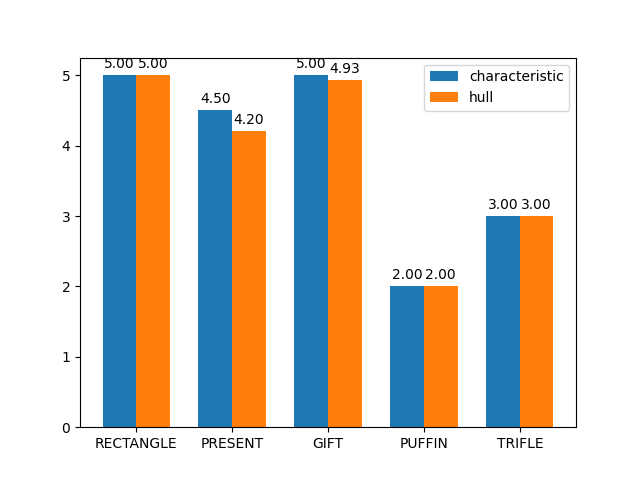
\includegraphics[width=1\textwidth]{fig/bar_ddt.png}
\end{figure}

\begin{figure}\label{fig:bar_lat2}
    \centering
    \caption{Results on iterative linear characteristics for some SPN block ciphers including RECTANGLE, PRESENT, GIFT64, PUFFIN, EPCBC and TRIFLE. The y-axis is the negative logarithm of linear correlation squares. The blue bars are the weight growth of the best iterative characteristics. The orange bars are the weight growth of the best iterative hulls.}
	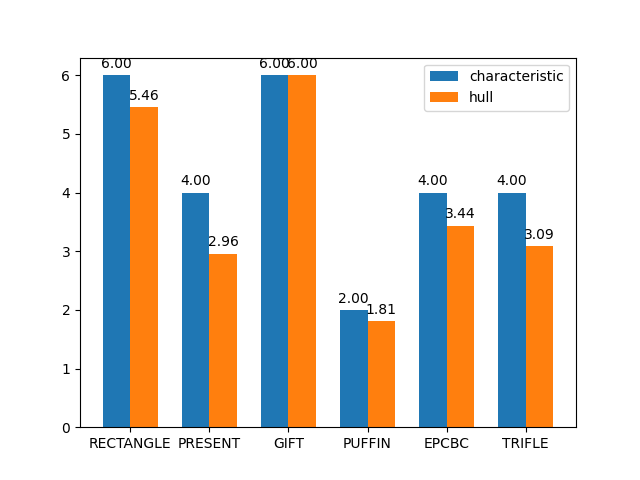
\includegraphics[width=1\textwidth]{fig/bar_lat2.png}
\end{figure}

In the following, we list the experimental settings for each of the primitive. 

\subsubsection{RECTANGLE} All operations of RECTANGLE has the rotational symmetry and thus we set the equivalance relation to be $=_R$. We set $A=3$ in both cases of differential and linear cryptanalysis. 

\subsubsection{PRESENT} We set $A=3$ in the differential case and $A=1$ in the linear case. 

\subsubsection{GIFT} We set $A=3$ in both differential and linear cases. 

\subsubsection{PUFFIN} We set $A=1$ in both differential and linear cases.

\subsubsection{EPCBC} We set $A=1$ in the linear case. We can't find any iterative characteristic though $A$ is set up to 3. 

\subsubsection{TRIFLE-BC} We set $A=1$ in both diffrential and linear cases. 

%\begin{figure}\label{fig:plot_ite}
%    \centering
%    \caption{Results on some SPN block ciphers, which are RECTANGLE, PRESENT, GIFT64, PUFFIN, EPCBC and TRIFLE from top to bottom resp. For each subfigure, the x-axis is the number of rounds. For a subfigure in the left column, the y-axis is the weight of differential probability, while for a subfigure in the right column, the y-axis is the weight of correlation square. The red spot denotes the best single iterative characteristic with fewest rounds obtained by Algo. \ref{algo:find_ite_c_G}. The yellow (green, blue) line denotes the best iterative hull with $A=$1 (2, 3).} 
%	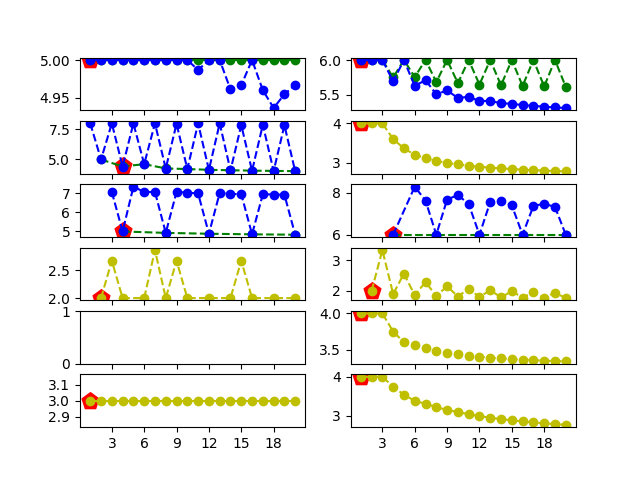
\includegraphics[width=1\textwidth]{fig/iterative.png}
%\end{figure}

\subsection{Results on Estimating EDPs and ELPs}

We apply our algorithm in Section \ref{sec:method-edp-elp} to some SPN primitives. The results are given in Table \ref{tab:EDP} and Table \ref{tab:ELP}. 

\begin{table}
	\caption{Results on estimating EDPs}\label{tab:EDP}
	\centering
	\begin{tabular}{|c|c|c|c|c|c|c|}
		\hline
		cipher & $r$ & $A$ & $(k,-\log_2wlb)$ & $-\log_2\Prob$ & $-\log_2\EDP$ & $T_g+T_s$ \\
		\hline
		PRESENT & 16 & 2 & (3,10) & 70 & 61.84 & 26s+165s\\
		\hline
		GIFT-64 & 13 & 2 & (3,13) & 62 & 60.42 & 24s+76s\\
		\hline 
		RECTANGLE & 14 & 2 & (6,25) & 61 & 60.65 & 4s+133.1h \\
		\hline
		KNOT-perm-256 & 52 & (2,*,1) & (3,12) & 274 & 251.831 & 0s+10s\\
		\hline
	\end{tabular}
\end{table}

\begin{table}
	\caption{Results on estimating ELPs}\label{tab:ELP}
	\centering
	\begin{tabular}{|c|c|c|c|c|c|c|}
		\hline
		cipher & $r$ & $A$ & $(k,-\log_2wlb)$ & $-2\log_2\Cor$ & $-\log_2\ELP$ & $T_g+T_s$ \\
		\hline
		PRESENT & 24 & 1 & (3,8) & 92 & 63.61 & 0s+14s\\
		\hline
		GIFT-64 & 13 & 2 & (3,10) & 64 & 64 & 1s+1s\\
		\hline 
		RECTANGLE & 14 & 3 & (3,14) & 68 & 62.31 & 17s+1.5h \\
		\hline
		KNOT-perm-256 & 56 & 3 & (2,6) & 161 & 125.262 & 27s+6.0h\\
		\hline
	\end{tabular}
\end{table}

\subsubsection{Comparison with the results in \cite{EPRINT:HalVej18}}



\subsection{Results on differential and linear attacks against KNOT-AEAD and KNOT-Hash}

\begin{table}
	\caption{Results for the primary version of KNOT}\label{tab:knot}
	\centering
	\begin{tabular}{|c|c|c|c|c|c|c|c|}
		\hline
		Attack Model & $r$ & $A$ & $(k,-\log_2wlb)$ & $-\log_2$(EDP or ELP)\\
		\hline
		AM1 & 14 & 2 & (5,20) & 62.2 \\
		AM2 & 13 & 3 & (3,8) & 30.7*2=61.4 \\
		AM3 & 12 & 3 & (3,10) & 30.2*2=60.4 \\
		AM4 & 12 & 2 & (5,20) & 62.4 \\
		AM5 & 13 & 2 & (5,20) & 61.4 \\
		AM6 & 12 & 2 & (5,20) & 62.7 \\
		AM7 & 13 & 2 & (5,20) & 61.4 \\
		\hline
	\end{tabular}
\end{table}

\subsubsection{Comparison with the method of enumerating characteristics}

\subsection{Visualization of the Iterative Structure}

\begin{figure}\label{fig:dis-rect}
    \centering
    \caption{Visualization of the differential iterative structure of RECTANGLE when $A=2$. The red part is the strong components. }
	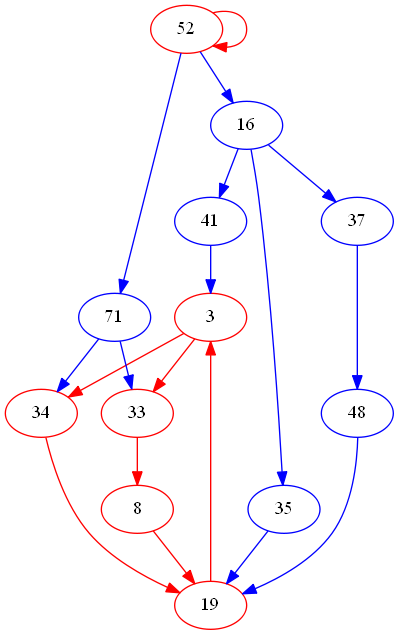
\includegraphics[width=0.5\textwidth]{fig/test_circuits.png}
\end{figure}

\begin{table}
	\caption{The differential iterative structure of RECTANGLE when $A=2$}\label{tab:dis-rect}
	\centering
	\begin{tabular}{|c|c|c|c|c|c|}
		\hline
		head No. & head difference & tail No. & tail difference & $d$ & $\Prob$ \\
		\hline
		3 & 8c00000000000000 & 33 & 3000c00000000000 & 0 & $2^{-5}$ \\
        3 & 8c00000000000000 & 34 & 3000800000000000 & 0 & $2^{-5}$ \\
        8 & 800000000000a000 & 19 & 500000000000000a & 0 & $2^{-6}$ \\
        16 & 6000000000000008 & 35 & 3000400000000000 & 15 & $2^{-5}$ \\
        16 & 6000000000000008 & 37 & 3000000000000000 & 15 & $2^{-5}$ \\
        16 & 6000000000000008 & 41 & 2300000000000000 & 14 & $2^{-5}$ \\
        19 & 500000000000000a & 3 & 8c00000000000000 & 2 & $2^{-5}$ \\
        33 & 3000c00000000000 & 8 & 800000000000a000 & 7 & $2^{-5}$ \\
        34 & 3000800000000000 & 19 & 500000000000000a & 4 & $2^{-6}$ \\
        35 & 3000400000000000 & 19 & 500000000000000a & 4 & $2^{-5}$ \\
        37 & 3000000000000000 & 48 & 2000800000000000 & 15 & $2^{-3}$ \\
        41 & 2300000000000000 & 3 & 8c00000000000000 & 3 & $2^{-6}$ \\
        48 & 2000800000000000 & 19 & 500000000000000a & 4 & $2^{-6}$ \\
        52 & 2000060000000000 & 16 & 6000000000000008 & 4 & $2^{-5}$ \\
        52 & 2000060000000000 & 52 & 2000060000000000 & 15 & $2^{-5}$ \\
        52 & 2000060000000000 & 71 & 2000000000000008 & 4 & $2^{-5}$ \\
        71 & 2000000000000008 & 33 & 3000c00000000000 & 15 & $2^{-6}$ \\
        71 & 2000000000000008 & 34 & 3000800000000000 & 15 & $2^{-6}$ \\
		\hline
	\end{tabular}
\end{table}